\subsection{Brief overview}

To start off, we summed up the total sales of all shops and items combined to get a feel of potential seasonal outliers as well as a general trend.

\begin{figure}[h]
  \centering
  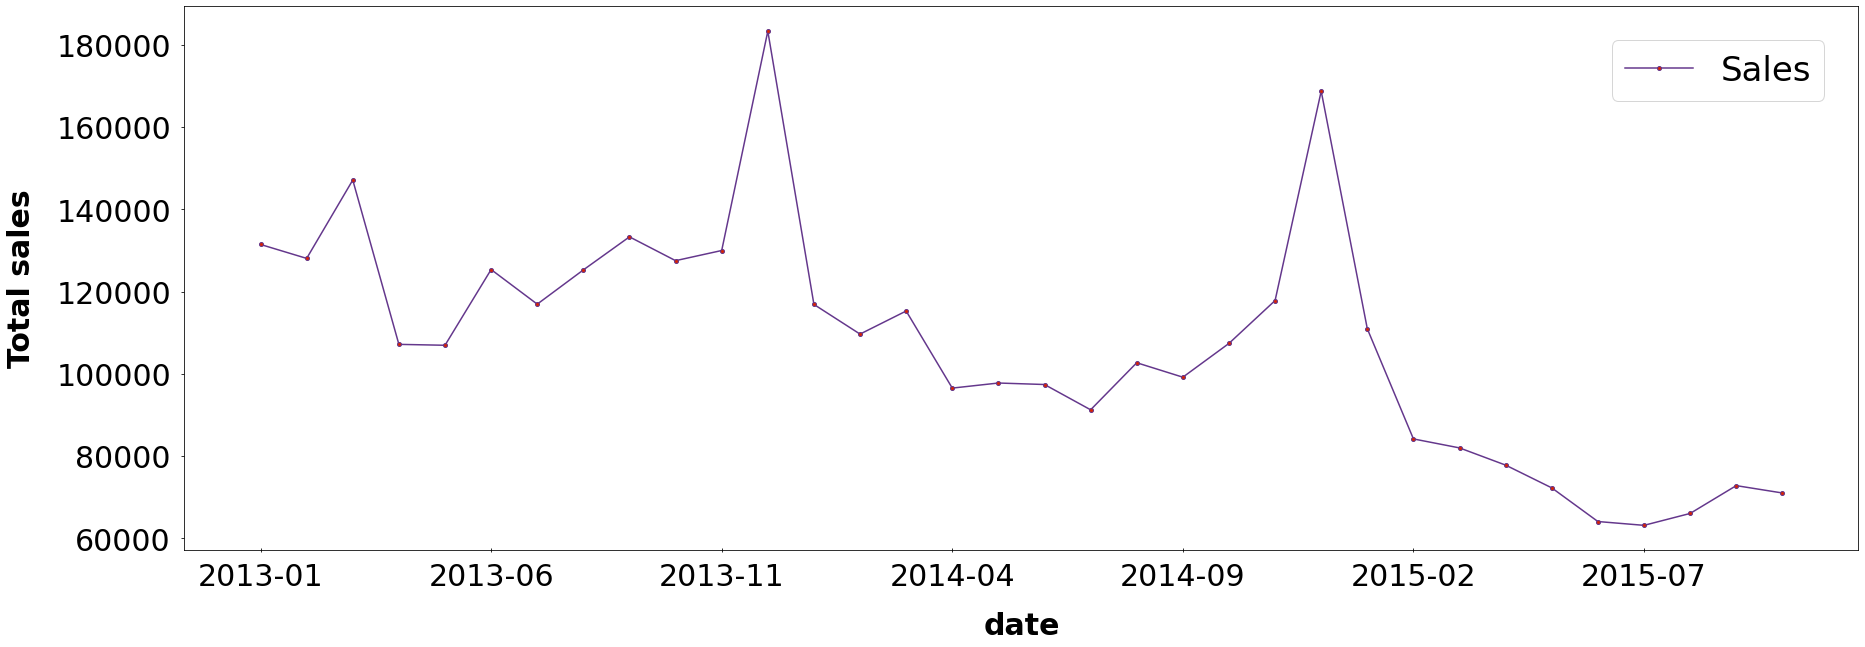
\includegraphics[width=0.9\linewidth]{external_content/graphs/total_sales.png}
  \captionsetup{justification=centering}
  \captionof{figure}{Total sales of the company}
  \label{fig:total_sales}
\end{figure}


We can observe that the sales peak in the month of December. This could be due to the increasing demand of gifts and disposable income from the population, but it could also indicate special Christmas sales which are common at this time of the year. Additionally, we observe a slight decline in demand over the timespan of the dataset.

To compare and validate the above statements, we plotted the total revenue of the company:

\begin{figure}[h]
  \centering
  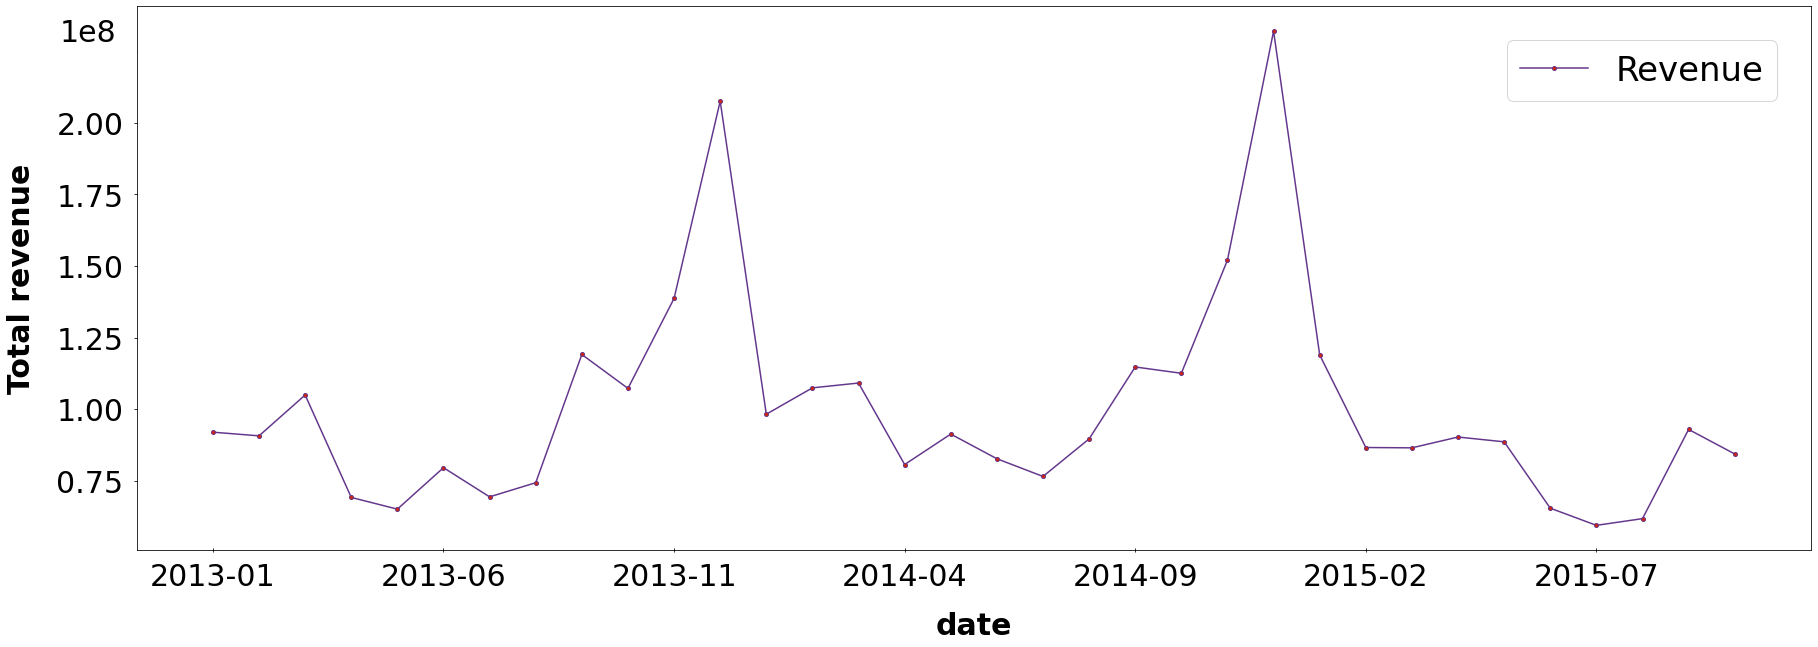
\includegraphics[width=0.9\linewidth]{external_content/graphs/total_revenue.png}
  \captionsetup{justification=centering}
  \captionof{figure}{Total revenue of the company}
  \label{fig:total_revenue}
\end{figure}

The seasonality of the data is clearly confirmed. Meanwhile, the downwards trend does not appear to be of particular relevance. The revenue stream has a constant trend over the years while having fewer sales. We should hereby be aware of the trend of having fewer sales with more expensive items.

To finish off the brief overview, we are taking a look at the correlation between the features and the label.

\begin{wrapfigure}{l}{0.6\textwidth}
\centering
  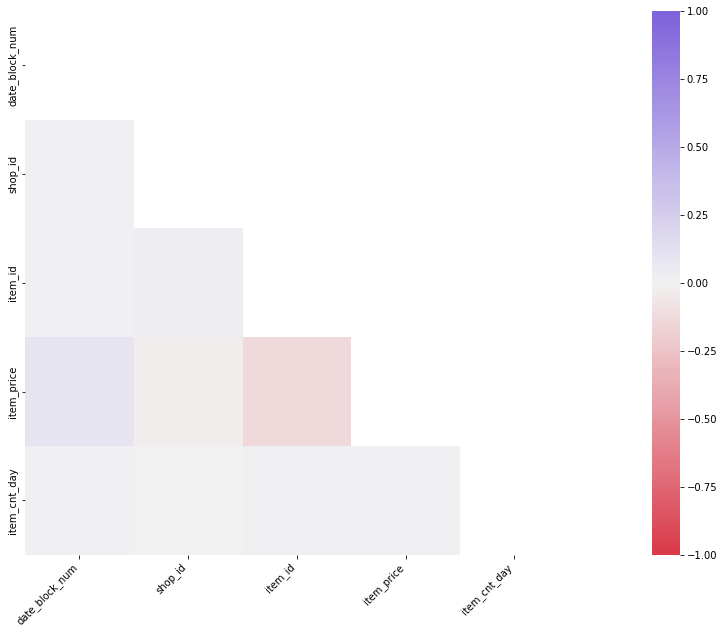
\includegraphics[width=0.9\linewidth]{external_content/graphs/corr_matrix.png}
\captionsetup{justification=centering}
\caption{Correlation matrix}
\label{corr_matrix}
\end{wrapfigure}

\noindent As we can observe, the label \texttt{item\_cnt\_day} has no strong correlation between any of the given features. 
This most likely leads to difficult to predict models, as no clear characteristics of the label is found in relation to the various features.

Additionally, no high correlation between features is observed. Therefore, we are not checking any features for multicollinearity at this point. \cite{MultivariateStatistics}

\clearpage